\documentclass{sig-alternate}
\usepackage[utf8]{inputenc}

\newcommand{\redcolor}[1]{\textcolor{red}{#1}}
\newcommand{\figref}[1]{Figure~\ref{#1}}
\newcommand{\secref}[1]{Section~\ref{#1}}
\newcommand{\tabref}[1]{Table~\ref{#1}}
\newcommand{\algoref}[1]{Algorithm~\ref{#1}}

\title{NILMTK: An open source toolkit for Non-intrusive load monitoring}
\author{Nipun Batra$^1$, Jack Kelly$^2$, Oliver Parson$^3$, Haimonti Dutta$^4$, William Knottenbelt$^2$,\\ Alex Rogers$^3$,Amarjeet Singh$^1$, Mani Srivastava$^5$\\
\scriptsize$^1$Indraprastha Institute of Information Technology, Delhi, India\\
\scriptsize\{nipunb,amarjeet\}@iiitd.ac.in\\
\scriptsize$^2$ Imperial College, London\\
\scriptsize\{jack.kelly@imperial.ac.uk, wjk@doc.ic.ac.uk\}\\
\scriptsize$^3$ University of Southampton\\
\scriptsize\{op106,acr\}@ecs.soton.ac.uk\\
\scriptsize$^4$ CCLS, Columbia\\
\scriptsize\{haimonti@ccls.columbia.edu\}\\
\scriptsize$^5$ UCLA\\
\scriptsize\{mbs@ucla.edu\}\\
}


\date{December 2013}

\begin{document}

\maketitle

\section{Abstract}
Non-intrusive load monitoring, or energy disaggregation, aims to separate household energy consumption data collected from a single point of measurement into individual appliances. In recent years, the field has rapidly increased in size with the national rollouts of smart meters, and as a result many new disaggregation algorithms have been proposed. However, empirically comparing such algorithms is currently virtually impossible, as a result of the different data sets used, the lack of availability of algorithms, and the wealth of accuracy metrics which have been employed. To address this challenge, we present NILMTK; an open source toolkit designed specifically to enable the comparison of energy disaggregation algorithms in a reproducible manner. Our toolkit includes parsers to a range of existing data sets, a standard output format for disaggregation algorithms, a set of statistics for describing datasets, a reference benchmark disaggregation algorithm, and a suite of accuracy metrics. We demonstrate that our toolkit lowers the barrier to entry by simplifying the use of multiple data sets, ease of adding new disaggregation algorithms, while also encouraging direct comparisons to be made between algorithms through common output formats and accuracy metrics.

\section{Introduction}
Non-intrusive load monitoring (NILM), or energy disaggregation, aims to break down a household's aggregate electricity consumption into individual appliances~\cite{hart_1992}. The motivations for such a process are threefold. First, informing a household's occupants of how much energy each appliance consumes empowers them to take steps towards reducing their energy consumption~\cite{darby_2006}. Second, 
personalised feedback can be provided which quantifies the savings of certain appliance-specific advice, such as the financial savings when an old inefficient appliance is replaced by a new efficient appliance. Third, if the NILM system is able to determine the time of use of each appliance, a recommender system would be able to inform the household's occupants of the potential savings through deferring appliance use to a time of day when electricity is either cheaper or has a lower carbon footprint.

Such benefits have drawn significant interest in the field since its inception 25 years ago. In recent years, the combination of national smart meter meter deployments (e.g. REF UK, USA) and also decreasing hardware costs of household electricity sensors has lead to a rapid expansion of the field. Such rapid growth over the past 5 years has been evidenced by the wealth of academic papers published, international meetings held (NLM 2012, EPRI NILM 2013), startup companies founded (e.g. Bidgely, Neurio) and data sets released.

However, three core barriers are currently preventing the direct comparison of existing approaches, and as a result are limiting progress within the field. First, each contribution to date has only been evaluated on a single data set as a result of the difficulty in moving from one data set to another, and consequently it is hard to assess the generalisability of approaches. Furthermore, many papers subsample existing data sets to select specific households, appliances and time periods, making experimental results harder to reproduce. Second, newly proposed approaches are rarely benchmarked against the same algorithms, further increasing the difficulty in empirical comparisons of performance between different papers. Moreover, the lack of availability of state-of-the-art algorithms often leads to the reimplementation of such approaches. Third, each paper targets a subtly different use case for NILM and therefore evaluates the accuracy of their proposed approach using a different set of performance metrics. As a result the numerical performance calculated by such metrics cannot be compared between two papers. These three barriers have led to successive extensions to state-of-the-art algorithms being proposed, while a direct comparison between such approaches has remained impossible.

Similar barriers also have arisen in other research fields and prompted the development of toolkits specifically designed to support a given area. For example, PhysioToolkit offers access to over 50 databases of physiological data and provides software to support the processing and analysis of such data for the biomedical research community~\cite{physionet}. Similarly, CRAWDAD collects 89 data sets of wireless network data in addition to supporting software to aid the analysis of such data by the wireless network community~\cite{crawdad}. However, no such toolkit is available to the NILM community.

Against this background, we propose NILMTK; an open source toolkit designed specifically to enable the comparison of energy disaggregation algorithms. The primary aim of the toolkit is to provide a complete pipeline from data sets to accuracy metrics, therefore lowering the barrier to entry for researchers to plug in a new algorithm and compare its performance to the current state of the art. The toolkit has been released as open source software in an effort to encourage researchers to contribute data sets, benchmark algorithms and accuracy metrics as they are proposed, with the goal of enabling a greater level of collaboration within the community. In addition, the toolkit has been designed using a modular structure, therefore allowing researchers to reuse or replace individual components as required. Last, the toolkit has been written in Python with flat file input and output formats, in addition to high performance binary formats, ensuring compatibility with existing algorithms written in any language and designed for any platform.

Our contributions are summarized as follows:\begin{itemize}
\item We propose REDD+, the standard structure for energy disaggregation data sets used by NILMTK based on an extension of the format used for the REDD data set. Furthermore, we provide parsers from multiple existing data sets into our proposed REDD+ format. In addition, we propose a single output format for the disaggregated data produced by NILM algorithms.
\item We provide an implementation of a benchmark disaggregation which uses combinatorial optimization to disaggregate household energy data into individual appliances. We demonstrate the ease by which NILMTK allows comparing this algorithm across a range of existing data sets, and present results of its performance accuracy.
\item We present a suite of accuracy metrics which are able to evaluate the performance of any disaggregation algorithms which produce output compatible with NILMTK. This allows the performance of a disaggregation algorithm to be evaluated for a range of use cases.
\end{itemize}
The remainder of this paper is organized as follows. In \secref{sec:related} we provide an overview of related work from the field of NILM and also other similar fields of research. In \secref{sec:nilmtk} we present NILMTK, and give a detailed description of its components. In \secref{evaluation} we demonstrate the empirical evaluations which are enabled by NILMTK, and provide analysis of existing data sets and accuracy metrics. Finally, in \secref{sec:conclusions} we conclude the paper and propose directions for future work.

\section{Related Work}
\label{sec:related}

\begin{table*}[]
  \centering
  \begin{tabular}{c c c c c c c c}
    \hline
    \bf Data set & \bf Institution & \bf Location & \bf Duration & \bf Number of & \bf Frequency of & \bf Aggregate\\
    \bf  & \bf  & \bf  & \bf  & \bf houses & \bf ground truth & \bf data available\\
    \hline
    REDD & MIT & MA, USA & 3-19 days & 6 & 3 second & Yes\\
    BLUED & CMU & PA, USA & 8 days & 1 & N/A & No\\
    Smart* & UMass & MA, USA & 3 months & 1 & 1 second & Yes\\
    Sample data set & Pecan Street & TX, USA & 7 days & 10 & 1 minute & Yes\\
    HES & DECC & UK & 3 months & 250 & 2 minute & No\\
    AMPds & Simon Fraser U. & BC, Canada & 1 year & 1 & 1 minute & Yes\\
    iAWE & IIIT Delhi & Delhi, India & 73 days & 1 & 1 second & Yes\\
    \hline
  \end{tabular}
  \caption{Table of comparison of household energy data sets.}
  \label{table:datasets}
\end{table*}

The field of non-intrusive load monitoring was founded over 20 years ago when Hart proposed the algorithmic disaggregation of household energy usage~\cite{hart_1992}. Since, many summary studies have shown the benefits of disaggregated data to both household occupants through financial savings, and also to utility providers through load shedding potential~\cite{zeifman_2011,armel_2013}. However, the majority of research had been evaluated using either lab-based data or simulated data, and as a result the performance of disaggregation algorithms in real households has remained unknown. More recently, national deployments of smart meters have prompted a renewed interest in energy disaggregation, and as a result a number of data sets collected specifically for energy disaggregation have been released. We now discuss the data sets which are currently available, which we subsequently summarise in \tabref{table:datasets}.

In 2011, the Reference Energy Disaggregation Dataset (REDD)~\cite{redd} was the first data set to be released which was collected specifically to aid NILM research. The data set contains both aggregate and sub-metered power data from 6 homes, and has since become the most popular data set for evaluating energy disaggregation algorithms. The following year, the Building-Level fUlly-labeled dataset for Electricity Disaggregation (BLUED) was released containing data from a single household. However, the data set does not include sub-metered power data, and instead events were recorded each time an appliance changed state (e.g.\ turned on). As a result, it is only possible to evaluate how well appliance activity can be inferred, rather than the disaggregation of appliance energy consumption. More recently, the SMART*~\cite{smart} data set was released, which contains household aggregate power data from 3 homes, while sub-metered appliance power data was only collected from a single household.

In 2013 the Pecan Street Sample data set was released~\cite{pecan}, which contains both aggregate data and sub-metered data from 10 households. Later, the Household Energy Study data set was released, which contains data from 250 households although only sub-metered appliance data was collected. Also that year, the Almanac of Minutely Power dataset (AMPds)~\cite{ampds} was released which contains both aggregate and sub-metered data from a single household. Most recently, the Indian data for Ambient Water and Electricity Sensing (iAWE)~\cite{iawe} was released, which contains both aggregate and sub-metered electricity data from a single home.

Unfortunately, subtle differences in the aims of each data set have lead to completely different data formats being used, and as a result a significant engineering barrier exists when moving from one data set to another. This has resulted in publications using only a single data set to evaluate a given approach, and consequently the generality of results are rarely investigated. Having described the data sets that are currently available, we now discuss recent publications which have used such data sets for the evaluation of disaggregation algorithms.

\section{NILMTK}
\label{sec:nilmtk}
We took the following three views/design goals while coming up with a design of NILM toolkit:
\begin{itemize}
\item \textbf{Analysis}: The toolkit should facilitate easy analysis of NILM datasets and expose the entire pipeline from
data importing to disaggregation and finally results. 
\item \textbf{Ease of adding new algorithms}: The toolkit should provide consistent interfaces for new disaggregation algorithms.
\item \textbf{Ease of deploying}: The toolkit should be built in such a way that the learnt model is easily deployable and can interface with online as well as offline data.
\end{itemize}
With these three design goals in mind, we decided to use Python as the programming language for building NILMTK

Python is increasingly becoming popular for Data Science, Machine Learning and open science. Python allows easy deployment in diverse environments including academic settings. The availability of a vast set of libraries varying from statistical analysis (Pandas), machine learning (Scikit-learn), web frameworks (Django), etc, make it a suitable choice for our project. Further, the availability of Python on platforms such as Raspberry Pi make it even more ideal.


\subsection{NILMTK pipeline}
In this section we describe the implementation and design of NILMTK pipeline. 
\subsubsection{Dataset Importers}A variety of datasets have been released in the recent time. The vast variety of formats in which these datasets are collected imposes limitations on the ease of NILM comparison. Motivated by this, we decided to import all the existing datasets into a common format based on the REDD format, which we call REDD+. We provide both CSV flat files based format and a much optimized Hierarchical Data Format (HDF5) based binary file format. At the time of writing, we have imported the following datasets in REDD+ format: REDD, PECAN, HES, iAWE, AMPds. In addition to storing electricity data, REDD+ format allows storing relevant metadata. For instance, if the electrical wiring is known, it can help in NILM. Further, if the geo coordinates of the building are known, it can help in correlating weather information and electricity usage.

\subsubsection{Preprocessing}Most of these datasets are collected using diverse hardware under different setting. For a valid comparison, these datasets must be preprocessed to common settings, such as sample size. Further, as proposed by Hart et. al~\cite{hart_1992}, voltage fluctuations significantly impact power draw. Techniques for voltage normalization are also presented in the preprocessing module.

$$P_{norm} = (\frac{V_{observed}}{V_{nominal}})^2.P_{observed}$$

\subsubsection{Statistics} 

\subsubsection{Training and Disaggregation}
We implement Combinatorial optimization based NILM. Its mathematical formulation is given as follows:


\subsubsection{Model exporting}

\subsubsection{Metrics}

\section{Evaluation}
\label{evaluation}
Dummy figure
\begin{figure}
\centering 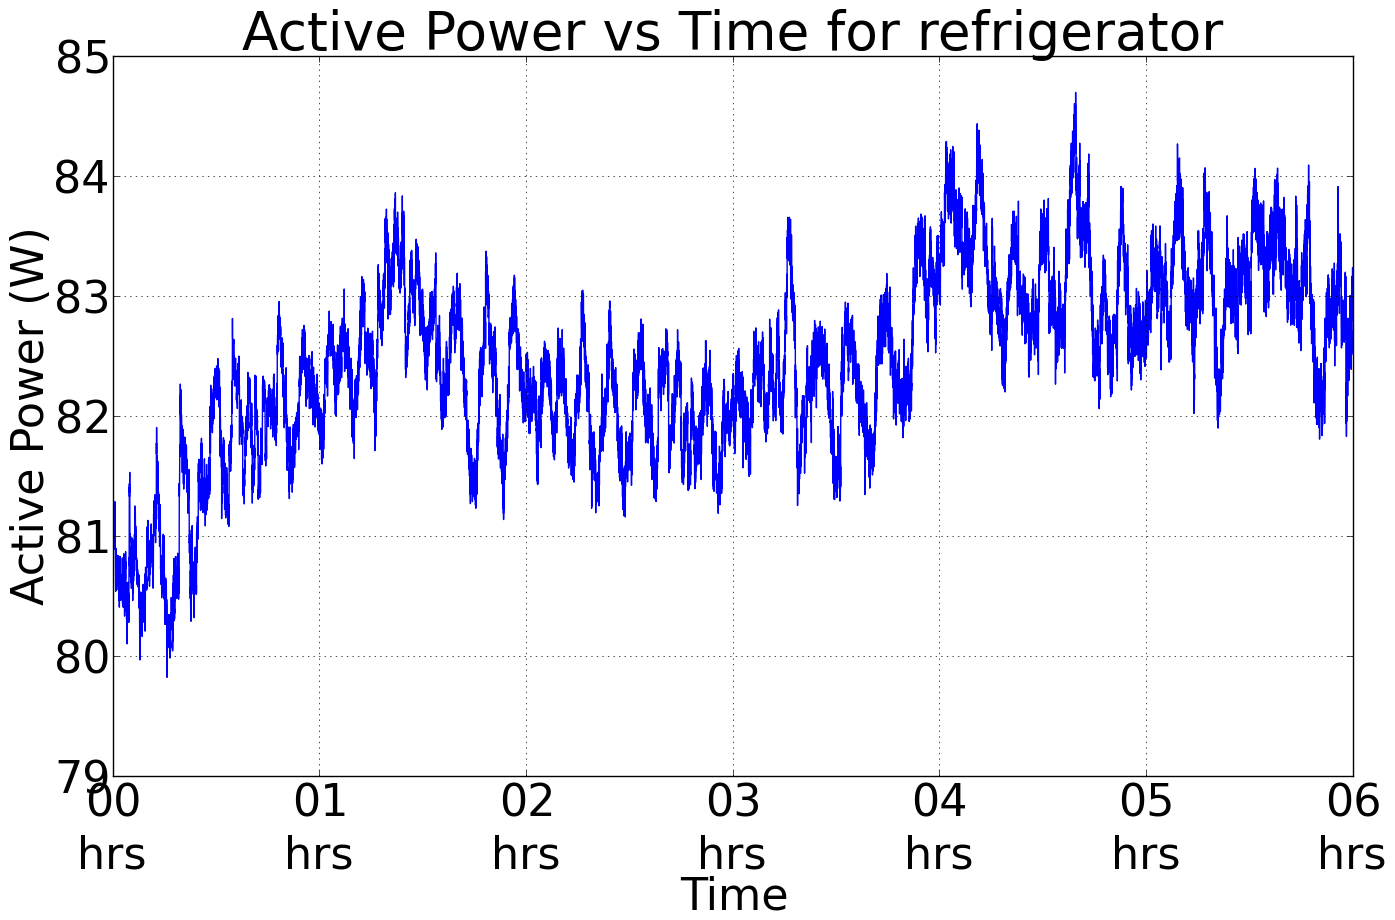
\includegraphics[scale=0.1]{figures/after_repair.png}
\caption{Dummy figure}
\label{fig:dummy}
\end{figure}


\begin{tabular}{|c|c|c|c|c|c|c|c|}
\hline
Appliance(n) & Main & \multicolumn{6}{|c|}{States Power (W)}\\
\hline
&&\multicolumn{3}{|c|}{Pre calibration}&\multicolumn{3}{|c|}{Post calibration}\\
\hline
             &  &$\mu^n_1$&$\mu^n_2$&$\mu^n_3$&$\mu^n_1$&$\mu^n_2$&$\mu^n_3$\\[0.1cm]
\hline
Refrigerator & 2& 7&162&423 & 7&214&423\\
%\footnote{There were not enough instances of refrigerator in state 3 to calibrate it}\\
Microwave &2& 9&822&1740& 9&822&1740\\
Lighting & 2& 9&96&156&9&113&156\\
Dishwasher & 1& 0&260& 1195 & 0&260& 1195\\
Stove& 1 & 0&373&-& 0&373&-\\
Kitchen & 1& 5&727&-&5&727&-\\
Kitchen 2&1 & 1&204&1036&1&204&1036 \\
%
%
\hline
%
\end{tabular}

\section{Discussion}

\section{Conclusions and future work}
\label{sec:conclusions}

\section{Acknowledgments}
The authors would like to thank TCS Research and Development for supporting the first author through PhD fellowship. We would also like to thank Department of Electronic and Information Technology (DEITy), Government of India for funding the project (Grant Number DeitY/R\&D/ITEA/4(2)/2012)
\bibliographystyle{abbrv}
\bibliography{reference}

\end{document}

